% CallVerse - technical report (Advanced Data Science Project, ESPRIT, 5DS3).
% Build:  latexmk -pdf main.tex   (or pdflatex, bibtex, pdflatex, pdflatex). Figures: python report/make_figures.py
\documentclass[11pt,a4paper]{article}

\usepackage[T1]{fontenc}
\usepackage[utf8]{inputenc}
\usepackage{lmodern}
\usepackage[a4paper,margin=2.2cm,headheight=14pt]{geometry}
\usepackage{microtype}
\usepackage{graphicx}
\usepackage{booktabs,tabularx,array,multirow}
\usepackage[table]{xcolor}
\usepackage{enumitem}
\usepackage{caption}
\usepackage{amsmath,amssymb}
\usepackage{fancyhdr}
\usepackage{tikz}
\usetikzlibrary{positioning,arrows.meta,fit,backgrounds,calc}
\usepackage[hidelinks]{hyperref}
\usepackage{url}

% ---------------------------------------------------------------- settings
\definecolor{cvblue}{HTML}{2A78D6}
\definecolor{cvink}{HTML}{1F2430}
\definecolor{cvmuted}{HTML}{5B6475}
\definecolor{cvline}{HTML}{E3E6EC}
\definecolor{cvsoft}{HTML}{F3F6FB}
\captionsetup{font=small,labelfont=bf,margin=0.5cm}
\setlist{itemsep=1pt,topsep=3pt,parsep=0pt}
\setlength{\parskip}{3pt}
\setlength{\emergencystretch}{2.5em} % lets lines with long code words break instead of overflowing
\renewcommand{\arraystretch}{1.12}
\newcolumntype{Y}{>{\raggedright\arraybackslash}X}
\newcommand{\code}[1]{\texttt{\small #1}}
\newcommand{\keyfig}[1]{\textbf{#1}}
% Fill in, then rebuild.
\newcommand{\tutor}{[Tutor's name]}
\newcommand{\demourl}{[public address, added once the Azure VM is online]}

\pagestyle{fancy}
\fancyhf{}
\fancyhead[L]{\small\color{cvmuted}CallVerse --- Technical report}
\fancyhead[R]{\small\color{cvmuted}5DS3 · ESPRIT}
\fancyfoot[C]{\small\thepage}
\renewcommand{\headrulewidth}{0.4pt}

\begin{document}

% ---------------------------------------------------------------- cover
\begin{titlepage}
  \centering
  \vspace*{0.6cm}
  {\large\textsc{ESPRIT School of Engineering}\par}
  \vspace{0.2cm}
  {\normalsize Advanced Data Science Project · Final assessment\par}
  \vspace{2.6cm}
  {\color{cvblue}\rule{\linewidth}{1.2pt}\par}
  \vspace{0.6cm}
  {\fontsize{40}{46}\selectfont\bfseries CallVerse\par}
  \vspace{0.4cm}
  {\Large A multi-agent digital twin of an\\[2pt] e-commerce customer service centre\par}
  \vspace{0.6cm}
  {\color{cvblue}\rule{\linewidth}{1.2pt}\par}
  \vspace{0.5cm}
  {\large Technical report\par}
  \vspace{2.4cm}
  \begin{tabular}{@{}l@{\hspace{1.2cm}}l@{}}
    \textbf{Group members} & Hamza Farhani \\
                           & Jihed Hmila \\
                           & Abdellaoui Woujoud \\
                           & Mohamed Aziz Kadri \\
                           & Mohamed Yessine El Ichi \\[8pt]
    \textbf{Class}         & 5DS3 \\[4pt]
    \textbf{Tutor}         & \tutor \\[4pt]
    \textbf{Date}          & 11 November 2026 \\
  \end{tabular}
  \vfill
  {\small\color{cvmuted} Academic year 2026--2027\par}
\end{titlepage}

% ---------------------------------------------------------------- abstract + contents
\section*{Abstract}
A customer service centre fails in two expensive ways: too few advisors when contacts spike, and too many
when it is quiet. Decisions about staffing and routing are usually tested directly on real customers.
\textbf{CallVerse} is a \emph{digital twin} of an e-commerce support centre: a virtual copy in which a manager
can test a decision before applying it. It forecasts contacts per reason from real order events (Olist, 99,441
orders), replays them in a discrete-event simulation, and lets four cooperating agents act inside it: a
\emph{Client} agent plays customers, a \emph{Workforce} agent routes chats and plans shifts, an
\emph{Advisor} agent answers with a retrieval-augmented language model and business tools, and a
\emph{Quality} agent grades every conversation. Each of our four data science objectives has a simple
baseline to beat, a backup, and a switch rule fixed in advance.
The forecast reduces the error of the naive baseline from 31.6\% to \keyfig{25.3\%} wMAPE, and the twin passes
every fidelity check. Shift planning with constraint programming cuts labour cost by \keyfig{40\%} while 92.4\%
of chats are still answered within 20 seconds (target 80\%). Testing a plan in the twin before a peak week cuts
understaffed hours by \keyfig{60--84\%}. Reinforcement-learning routing reduces the speed of answer by 13.9\% on
unseen stressed days but is not robust in full peak weeks, so a tuned rule stays in production.
Semantic retrieval raises recall@4 from 80.4\% to \keyfig{96.9\%}; the advisor that lets a rules engine decide and the
language model write gives 12/12 verified policy-correct actions, while the automatic judge is not yet
trusted (kappa below 0.4). The application (two web apps, an API, an MCP server and a live contact-centre
view) ships as one Docker container, with 200 automated tests and one command to reproduce every result.

\vspace{0.3cm}
\setcounter{tocdepth}{1}
{\small\tableofcontents}
\clearpage

\section{Introduction and problem statement}
\label{sec:intro}

\subsection{Context: an e-commerce customer service centre}
Most contacts to an online shop's customer service are caused by orders: a parcel is late (``where is my
order?''), a customer wants to cancel or get a refund, an item arrives damaged or wrong, or an invoice or
address must be changed. These causes are largely \emph{predictable}: the number of orders, the promotion
calendar and the carriers' delays are known days in advance. Yet many centres still plan from last year's
averages and react to peaks when they happen. This status quo has four costs:
\begin{itemize}
  \item \textbf{Peaks hurt customers}: long waits, abandoned chats, repeat contacts and bad reviews.
  \item \textbf{Quiet periods waste money}: staffing is the largest cost of a contact centre, and paid advisors
        sit idle.
  \item \textbf{Decisions are tested on real customers}: there is no safe place to ask ``what if a promotion
        doubles the tracking questions?'' or ``what if 20\% of the advisors are sick?''.
  \item \textbf{AI assistants are adopted without measurement}: chatbots answer customers, but few companies
        check whether the answers follow the company policy, or whether an automatic grader agrees with humans.
\end{itemize}

\subsection{Our answer: a digital twin with four agents}
CallVerse is a \emph{digital twin} of such a centre: a virtual copy that behaves like the real one, so that
a decision can be tested in seconds before customers feel it. The twin is driven by real e-commerce data
(the Olist marketplace) and is used by four cooperating \emph{agents}, programs that observe a situation and
act on it:
\begin{itemize}
  \item the \textbf{Client agent} plays customers, each with a real order, a problem and a personality;
  \item the \textbf{Workforce agent} recognises each customer's problem, sends the chat to the right advisor,
        and plans the advisors' shifts;
  \item the \textbf{Advisor agent} answers, using the company's policy documents and business tools (order
        lookup, refund eligibility, tickets);
  \item the \textbf{Quality agent} grades every conversation on a five-criterion scorecard.
\end{itemize}

\subsection{Business and data science objectives}
We framed the project as four \emph{business objectives} (BO), each measured by business KPIs, and four
\emph{data science objectives} (DSO), each measured by a model metric (Table~\ref{tab:bodso}). A KPI tells
whether the centre is doing better; a DSO metric tells whether the AI component works. Three rules apply to
every objective: (1) the main idea must beat a \emph{simple baseline}; (2) a \emph{backup} covers the whole
objective with less effort; (3) a \emph{switch rule}, fixed before the experiments, decides whether the main
idea or the backup goes to production. DSO4 is the foundation: DSO1 and DSO3 are trained and tested inside
its simulation.

\begin{table}[h]
\centering\small
\caption{From business objectives to data science objectives. ``Rule'' is the switch rule decided in advance.}
\label{tab:bodso}
\begin{tabularx}{\textwidth}{@{}p{2.5cm}YYYp{3.1cm}@{}}
\toprule
\textbf{Business objective} & \textbf{DSO and main idea} & \textbf{Baseline} & \textbf{Backup} & \textbf{Rule} \\
\midrule
BO1 Customers wait less & DSO1: real-time routing learned by reinforcement learning (MaskablePPO) &
  First come, first served (FIFO) with skill matching & Priority score with tuned weights &
  $\geq$10\% less waiting in the twin's peak weeks \\
BO2 Problems solved correctly, higher satisfaction & DSO2: advisor with retrieval-augmented generation and
  tools, plus an LLM judge & Keyword FAQ search; templates & Intent classifier + approved templates +
  checklist reviewer & $\leq$10\% wrong answers; judge--human kappa $\geq$ 0.4 \\
BO3 Lower cost, same service & DSO3: forecast + constraint-programming shift planning (CP-SAT) &
  Fixed schedule sized for the peak & Erlang C + shift templates + overtime rule &
  $\geq$5\% cheaper while meeting the service target and the labour rules \\
BO4 Prepare for peaks by testing first & DSO4: contact forecast per reason + discrete-event simulation &
  Same day last week; Erlang C queueing formula & Statistical forecast + queueing model &
  Beat the naive forecast; the twin passes its fidelity checks \\
\bottomrule
\end{tabularx}
\end{table}

\paragraph{What success means.} The centre's service target is the industry's ``80/20'' rule: 80\% of chats
answered within 20 seconds. A good plan meets it at the lowest labour cost and respects labour law (at most
5 days and 40 hours a week, at least 11 hours of rest between two shifts). A good answer applies the company
policy (for example: a parcel more than 7 days late triggers a carrier investigation) and leaves the customer
satisfied. Every claimed gain must be measured against its baseline on the same simulated customers, with a
95\% confidence interval.

\subsection{Contributions and structure of the report}
We deliver (1) a reproducible data pipeline from raw Olist and Bitext files to a relational store and a
knowledge base; (2) a forecast and a validated simulation engine; (3) four agents combining machine learning,
reinforcement learning, optimisation and language models; (4) an evaluation framework with paired
experiments, a scorecard and live monitoring of every AI component; and (5) a deployed application.
Section~\ref{sec:data} presents the data, Section~\ref{sec:method} the methods and architecture,
Section~\ref{sec:experiments} the experimental protocol and Section~\ref{sec:results} the results.
Section~\ref{sec:analysis} discusses limitations, Section~\ref{sec:deployment} deployment and
reproducibility, and Section~\ref{sec:aiuse} declares our use of generative AI tools.

\section{Data}
\label{sec:data}

\subsection{Sources}
No public contact-centre logs exist, so we combine two public datasets with real behaviour and a documented
generation step (Table~\ref{tab:sources}).
\begin{itemize}
  \item \textbf{Olist Brazilian e-commerce dataset}~\cite{olist}: 99,441 real, anonymised orders placed
        between 4 September 2016 and 17 October 2018, with items, payments, reviews, customers, sellers,
        products and every delivery timestamp (purchase, approval, carrier hand-off, delivery, estimate).
        Licence CC BY-NC-SA 4.0.
  \item \textbf{Bitext retail e-commerce customer-service dataset}~\cite{bitext}: 44,884 customer messages
        labelled with 46 intents (a customer's goal, such as \code{track\_order}). We keep the
        \textbf{17 intents linked to an order}, grouped into four families: \emph{where is my order}
        (wismo, 4 intents), \emph{cancel/refund} (3), \emph{after delivery} (7) and \emph{order admin} (3).
        Licence CDLA-Sharing 1.0.
  \item \textbf{Knowledge base}: 10 policy documents written for the project (refunds, returns, delivery
        delays, payments, invoices, an advisor playbook...), split into 58 sections.
\end{itemize}

\begin{table}[h]
\centering\small
\caption{Data used by CallVerse (SQLite store and processed tables).}
\label{tab:sources}
\begin{tabularx}{\textwidth}{@{}lrY@{}}
\toprule
\textbf{Table} & \textbf{Rows} & \textbf{Origin and use} \\
\midrule
Orders / customers & 99,441 & Olist; order situation, delivery dates, the advisor's order lookup \\
Order items / payments & 112,650 / 103,886 & Olist; refund amounts, payment anomalies \\
Products / sellers & 32,951 / 3,095 & Olist; product and seller context \\
Reviews & 99,224 & Olist; satisfaction signal during exploration \\
Contacts / tickets & 9,179 / 9,179 & Generated from the orders' situations (Section~\ref{sec:synthetic}) \\
Chat messages & 60,837 & Generated, with the wording of real Bitext messages \\
Knowledge-base sections & 58 & 10 policy documents, embedded with bge-m3 \\
\bottomrule
\end{tabularx}
\end{table}

\subsection{Exploration and quality validation}
Exploration (notebooks 01--02) confirmed that the orders are suitable: 97.0\% are delivered, 1.1\% shipped,
0.6\% cancelled and 0.6\% unavailable. All orders have a purchase time and an estimated delivery date; the
actual delivery time is missing for 2,965 orders, the carrier hand-off for 1,783 and the approval for 160,
which matches their statuses (an undelivered order has no delivery time). Review comments are often empty
(58.7\% have no message), and 610 products (1.9\%) have no category.

The quality validation found five kinds of contradictions (Table~\ref{tab:quality}). One correction matters for
the whole project: the estimated delivery dates are stored at midnight, so comparing them with a delivery
\emph{timestamp} counted orders delivered later on the same day as ``late''. Measured by calendar date,
\textbf{6,535 of 96,476 delivered orders (6.8\%) are late}, not the 7,826 reported in a first version.

\begin{table}[h]
\centering\small
\caption{Data quality findings. Each anomaly becomes a Boolean flag column; no row is deleted or imputed.}
\label{tab:quality}
\begin{tabularx}{0.8\textwidth}{@{}Yr@{}}
\toprule
\textbf{Finding (flag column)} & \textbf{Orders} \\
\midrule
Carrier hand-off before payment approval & 1,359 \\
Delivery before carrier hand-off & 23 \\
Review created before the purchase date (40 of them reuse a review id) & 64 \\
Order with more than one review & 547 \\
Payment total differs from items + freight by more than 1 BRL & 249 \\
\bottomrule
\end{tabularx}
\end{table}

\subsection{Cleaning and feature preparation}
Cleaning (notebooks 03--04) parses types and \emph{flags} anomalies rather than deleting them, so record
counts are preserved and no value is invented by imputation. It produces an \textbf{analytical order table of
77 features} (delivery delay, lateness, payment anomalies, review score, product and seller context...) and a
daily activity table (orders purchased, handed to carriers, delivered, delivered late). Six tables that later
layers depend on are protected by \emph{data contracts}: Pandera schemas~\cite{pandera} check keys, types,
allowed values and ranges (\code{callverse validate}); all pass.

\subsection{Synthetic contacts, tickets and chats}
\label{sec:synthetic}
Real contact logs are private, so contacts are generated from the real orders with explicit, documented
assumptions (\code{configs/data.yaml}, notebooks 05--08 and 12):
\begin{enumerate}
  \item Each order is placed in a \emph{situation}: never delivered and overdue, delivered late, cancelled,
        problem after delivery, payment anomaly, or uneventful.
  \item Each situation has a \emph{contact probability} (for example, 35\% of late deliveries contact
        support), an \emph{intent mix}, and a \emph{timing rule} relative to an order event (a delay-related
        contact comes after the estimated date has passed). Contact hours follow the hour-of-day profile of
        Olist purchases, and a promotion calendar adds known retail events.
  \item The customer's opening message is a real Bitext message of the chosen intent.
\end{enumerate}
The result is \textbf{9,179 contacts} from January 2017 to August 2018. We cross-checked the volume against a
public benchmark (``where is my order'' contacts at 3--10\% of orders). Each contact then becomes a ticket with
an outcome decided by the company rules (resolved in the chat 53.4\%, follow-up needed 43.4\%, escalated
3.2\%), a handle time drawn from the simulation's assumptions, and a satisfaction survey answered 30\% of the
time (mean 3.93/5). The \textbf{60,837 chat messages} use approved answer templates. All generated records carry
an \code{is\_synthetic} flag. Generation is seeded, so it is reproducible.

\subsection{Ethics, licences and confidentiality}
Olist identifiers are already anonymised, and no personal data is collected. Synthetic records are flagged
and the rates behind them are written in one configuration file, so they can be replaced by a client's real
logs without code changes. We respect the licences: non-commercial, share-alike use of Olist (CC BY-NC-SA 4.0)
and Bitext (CDLA-Sharing 1.0). The advisor never asks for card numbers or passwords (a prompt rule and a
checklist item), customers are told they talk to an AI, and staffing recommendations remain human decisions.
For the public deployment, a script removes the customers we created while testing (our own names) and the
transcripts of our test chats before anything leaves the laptop (Section~\ref{sec:deployment}).

\section{Methodology and architecture}
\label{sec:method}

\subsection{Process and architecture}
We followed CRISP-DM~\cite{crispdm}: business understanding (the BO/DSO framework), data understanding and
preparation (Section~\ref{sec:data}), modelling (forecast, twin, agents), evaluation (Section~\ref{sec:experiments})
and deployment (Section~\ref{sec:deployment}). The code is organised in five layers (Figure~\ref{fig:arch}). A
lower layer never imports a higher one; six \code{import-linter} contracts enforce this in the test suite.

\begin{figure}[h]
\centering
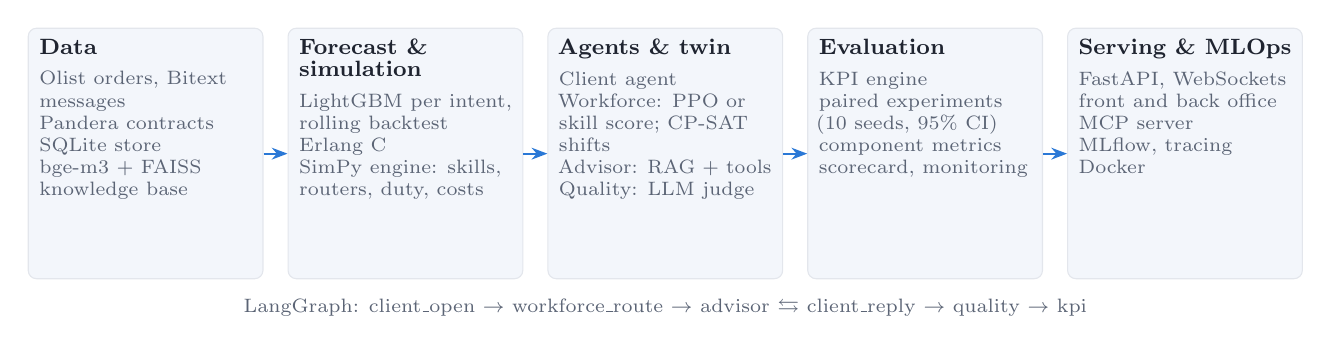
\begin{tikzpicture}[
  layer/.style={draw=cvline, fill=cvsoft, rounded corners=3pt, anchor=north, inner sep=4pt,
                font=\scriptsize, text=cvmuted},
  arrow/.style={-{Stealth[length=2mm]}, thick, draw=cvblue}]
  \foreach \i/\t/\body in {
    0/{Data}/{Olist orders, Bitext messages\\Pandera contracts\\SQLite store\\bge-m3 + FAISS knowledge base},
    1/{Forecast \& simulation}/{LightGBM per intent, rolling backtest\\Erlang C\\SimPy engine: skills, routers, duty, costs},
    2/{Agents \& twin}/{Client agent\\Workforce: PPO or skill score; CP-SAT shifts\\Advisor: RAG + tools\\Quality: LLM judge},
    3/{Evaluation}/{KPI engine\\paired experiments (10 seeds, 95\% CI)\\component metrics\\scorecard, monitoring},
    4/{Serving \& MLOps}/{FastAPI, WebSockets\\front and back office\\MCP server\\MLflow, tracing\\Docker}}{
    \node[layer] (L\i) at (\i*3.3, 0)
      {\parbox[t][2.9cm][t]{2.7cm}{\raggedright\hyphenpenalty=10000
        {\footnotesize\bfseries\color{cvink}\t}\\[3pt]\body}};
  }
  \foreach \a/\b in {0/1,1/2,2/3,3/4} { \draw[arrow] (L\a.east |- 0,-1.6) -- (L\b.west |- 0,-1.6); }
  \node[font=\scriptsize, text=cvmuted, align=center] at (6.6,-3.55)
    {LangGraph: client\_open $\rightarrow$ workforce\_route $\rightarrow$ advisor $\leftrightarrows$ client\_reply
     $\rightarrow$ quality $\rightarrow$ kpi};
\end{tikzpicture}
\caption{The five layers of CallVerse. Arrows show the only allowed direction of dependencies.}
\label{fig:arch}
\end{figure}

\subsection{DSO4, part 1: forecasting the contacts}
\textbf{Target.} Daily contacts per intent family (four series) and their total, 1 to 7 days ahead.
\textbf{Features.} Every feature is lagged by at least 7 days, so the model never sees the future (a unit test
checks it): the series' own history (lags 7, 14, 21 and 28 days, same-weekday mean, 7- and 28-day means),
\emph{order drivers} (orders purchased, handed to carriers, delivered and delivered late, orders promised for
the day, overdue backlog) and the calendar (weekday, holidays, promotion windows, days since the last major
sale). \textbf{Models.} The DSO baseline ``same day last week'' (seasonal naive), a 4-week weekday mean,
SARIMA(1,1,1)(0,1,1)$_7$~\cite{hyndman}, Prophet with holidays and promotions~\cite{prophet}, and one global
LightGBM~\cite{lightgbm} with a Poisson objective and the family as a categorical feature. The error measure
is the weighted mean absolute percentage error, which stays defined on days with few contacts:
\begin{equation}
\text{wMAPE} = \frac{\sum_t |y_t - \hat{y}_t|}{\sum_t y_t}.
\end{equation}

\subsection{DSO4, part 2: the digital twin}
The twin is a discrete-event simulation written with SimPy~\cite{simpy}. Customers arrive as a
non-homogeneous Poisson process: the daily volume (history or forecast) is spread over the hours with the
observed hourly profile, and scaled $\times$25 to represent a mid-size centre. Each customer has an intent
family, a lognormal handle time (means 3, 4, 6 and 7 minutes by family, coefficient of variation 0.6) and a
persona that sets its patience (impatient 25\%, normal 55\%, patient 20\%; mean patience 90, 180 and 360 s).
Advisors have skills: 0.75$\times$ the handle time on their main family, 1.3$\times$ on a weak one. A duty
matrix says who works each hour (regular or overtime) and a \emph{router} decides who serves whom. Chats that
arrive while the centre is closed (22:00--08:00) wait as an overnight backlog. Costs are €12 per hour, overtime
$\times$1.5, and €8 per abandoned customer. The engine has two modes: a full run for evaluation, and a
step-by-step mode that pauses at every routing decision for reinforcement learning.

\textbf{Validation against queueing theory.} With one skill and FIFO routing, the twin must reproduce the
\emph{Erlang C} model~\cite{gans}, which gives the probability that a customer waits when $c$ advisors serve
an offered load $A = \lambda \cdot \text{AHT}$:
\begin{equation}
P_{\text{wait}} = \frac{\frac{A^c}{c!}\frac{c}{c-A}}{\sum_{k=0}^{c-1}\frac{A^k}{k!} + \frac{A^c}{c!}\frac{c}{c-A}},
\qquad
\text{SL}(t) = 1 - P_{\text{wait}}\, e^{-(c-A)\,t/\text{AHT}}.
\end{equation}
\textbf{Scenarios} change a real week of history: a promotion spike (all families $\times$1.4--1.8), delivery
delays (wismo $\times$2.5, handle time +10\%), a staff shortage (20\% absent), and the real busiest week after
Black Friday 2017 (18 December 2017, about three times a normal November week, no multiplier).

\subsection{DSO3: shift and overtime planning}
From the forecast, Erlang C gives the number of advisors needed each hour to answer 80\% of chats within
20 s with an occupancy of at most 90\%. A two-stage model solved with OR-Tools CP-SAT~\cite{ortools} turns this
requirement into a roster.
\emph{Stage 1, cheapest coverage}: integer variables $x_{d,t}$ (advisors on shift template $t$ on day $d$;
27 templates of 4, 6 or 8 hours inside 08:00--22:00), $o_{d,h}$ (overtime advisors, at most 4 per hour and 60
hours per week) and $s_{d,h}$ (shortfall), with
\begin{equation}
\min \sum 12\,x\,\ell_t + 18\,o + 200\,s \quad \text{s.t.} \quad \sum_{t \ni h} x_{d,t} + o_{d,h} + s_{d,h}
\geq r_{d,h}\;\; \forall d,h,
\end{equation}
where $\ell_t$ is the template length and $r_{d,h}$ the requirement. \emph{Stage 2, legal roster}: Boolean
variables assign the chosen shifts to named advisors with one shift per day, at most 5 days and 40 hours per
week, and at least 11 hours of rest; the headcount grows until a solution exists. Both stages solve to
optimality in under a second; the solver runs on one thread so that the roster is reproducible.

\subsection{DSO1: real-time routing}
Routing is a sequential decision problem, written as a Markov decision process. \emph{Decision point}: an
advisor becomes free while at least two customers wait. \emph{State}: the 10 oldest waiting customers (time
waited, family, persona, live chat or overnight message, expected handle time with \emph{this} advisor), the
queue length, the backlog, free and on-duty advisors and the time of day. \emph{Action}: which waiting
customer to serve; empty slots are masked. \emph{Reward}: minus the customer-seconds of waiting since the last
decision (overnight messages weighted 0.1), minus 600 per abandonment. By Little's law~\cite{little},
minimising total waiting minimises the mean wait.
We train MaskablePPO~\cite{ppo,masking} (Stable-Baselines3~\cite{sb3}, Gymnasium~\cite{gymnasium}) on single
days of February 2017--March 2018 made busier than planned (load $\times$1.0--1.8, each family surging
$\times$1.0--1.6, 5--30\% absences): 2,394 episodes, 300,000 decisions, a 128$\times$128 network.
\textbf{Backup}: a priority score $w_1\,\text{wait} + w_2\,\text{skill match} + w_3\,\text{short job} +
w_4\,\text{impatient}$, whose weights are tuned by random search in the twin (best: 0.19, 1.80, 2.69, 0.08).

\subsection{DSO2: the language agents}
\textbf{Workforce agent (routing a chat).} A TF-IDF + logistic-regression classifier~\cite{sklearn} predicts the
intent of the first message (99.0\% accuracy, macro-F1 0.991 on 1,602 held-out Bitext messages) and sends the
chat to an advisor of that family, with the expected wait from Erlang C.

\textbf{Advisor agent.} The loop is: understand the request, retrieve the relevant policy, call tools, write
the reply. \emph{Retrieval}: bge-m3~\cite{bgem3} embeddings (multilingual, 1,024 dimensions) of the 58
knowledge-base sections in an exact FAISS index~\cite{faiss}; the top 3 sections are kept, with a ``no answer''
threshold at a cosine of 0.57. This is retrieval-augmented generation (RAG)~\cite{rag}: the model writes from
retrieved evidence instead of from memory. \emph{Tools} work on the SQLite store, ``as of'' the moment the
customer writes: \code{lookup\_order}, \code{get\_ticket\_history}, \code{check\_refund\_eligibility},
\code{open\_ticket}, \code{search\_knowledge\_base} and the company rules engine \code{recommend\_resolution}. We
compare four variants:
\begin{itemize}
  \item \textbf{template} (backup): the classifier's intent selects an approved answer filled with order facts;
  \item \textbf{rag} (pure idea A): the LLM decides which tools to call and writes freely;
  \item \textbf{rag\_policy} (hybrid): once the order number is known, the pipeline itself calls
        \code{lookup\_order} and the rules engine; the LLM receives the decision and only \emph{writes} it;
  \item \textbf{agentic}: the hybrid plus tools the LLM chooses itself, in a ReAct-style loop~\cite{react}: a
        reflection step that fact-checks the draft against the data (\code{check\_draft\_reply}), a hand-off
        to a human (\code{escalate\_to\_human}), a check of bank codes against a public list
        (\code{validate\_bank\_code}) and a memory of earlier contacts (\code{get\_customer\_history}).
\end{itemize}
The first LLM runs exposed failure modes that we turned into guardrails: the model called \code{lookup\_order}
with invented ids (9 of 20 calls failed), so order tools are only offered once an order number appears in the
chat (\emph{tool gating}); it sometimes answered before checking the order, so a reply given before
verification always ends with the order-number request. LLM-chosen tool calls go through our
\textbf{Model Context Protocol} (MCP)~\cite{mcp} server, which outside applications can also use.

\textbf{Client agent.} It plays the customer of a real contact (opening message, persona, knowledge of its
order) and ends with a 1--5 satisfaction score. It has three tools of its own: \code{view\_my\_order\_page} (to
check a status or date the advisor states), \code{check\_my\_waiting\_time} (its patience budget) and
\code{send\_evidence} (photos or a payment statement, built from the real order, never written by the LLM).

\textbf{Quality agent.} A scorecard of five criteria rated 1--5 (compliance, relevance, satisfaction,
sentiment, resolution), filled by an LLM judge~\cite{llmjudge} from a \emph{different model family} than the
advisor, to avoid a model grading its own style. The judge receives the policy-correct reference. A
rule-based checklist is the offline backup. Correctness is also measured \emph{deterministically}: the action
chosen by the advisor must equal the action the rules give for the true intent.

The agents are chained with LangGraph~\cite{langgraph}, whose state (messages, routing decision, reference,
scorecard, KPIs) is streamed step by step to the user interface.

\subsection{LLM setup: three tiers}
\label{sec:llmsetup}
Every agent works at three levels, so the twin never stops:
\begin{enumerate}
  \item \textbf{Hosted open models through OpenRouter (main, since 3 November 2026)}, free tier: NVIDIA
        Nemotron 3.5 Super for the advisor, Nemotron 3.5 Lightning for the client, and Xing 4.0 (another
        family) for the judge, each with a fallback model. Reasoning mode is switched off: these models
        otherwise returned empty answers. The free tier allows 20 requests per minute and 50 per day; when the
        daily quota is used, OpenRouter is skipped until 00:00 UTC.
  \item \textbf{Local Hugging Face models (backup)}: SmolLM3-3B (advisor, client) and IBM Granite-4.0-1B
        (judge), quantised to 4 bits so that both fit the 4 GB laptop GPU (GTX 1650). Model commits are pinned.
  \item \textbf{Offline templates and rules}: the template advisor, the rule-based customer and the checklist.
\end{enumerate}
We moved from local to hosted models after measuring them: a local advisor call took 16 s at the median
because the 4 GB GPU overflowed into shared memory, against about 2 s on OpenRouter (Section~\ref{sec:monitoring}).
All calls are cached (SQLite) and traced (one JSON line per call: model, tokens, latency, tools, cost).

\section{Experiments}
\label{sec:experiments}

\subsection{Principles}
Every experiment runs from one command (\code{callverse evaluate}) and writes its tables to
\code{artifacts/evaluations/}, with a summary run in MLflow~\cite{mlflow}. Four principles apply throughout:
\begin{itemize}
  \item \textbf{A baseline and a backup for every idea}, and a switch rule fixed \emph{before} the results are
        known (Table~\ref{tab:bodso}). The scorecard (\code{scorecard.json}) applies these rules automatically.
  \item \textbf{Common random numbers}~\cite{law}: every option is simulated on exactly the same random
        customers (arrivals, handle times, patience), so a difference comes from the decision only.
  \item \textbf{Paired differences with 95\% Student-t confidence intervals} over seeds; a difference is called
        \emph{significant} only when its interval excludes zero.
  \item \textbf{No leakage}: models are trained on the past only (rolling origins for the forecast, a training
        period before a test period for routing).
\end{itemize}

\subsection{Experiments and protocols}
Table~\ref{tab:experiments} lists the experiments. Simulated weeks use 10 seeds; the routing study on stressed
days uses 20 unseen days with 2 seeds each (40 pairs).

\begin{table}[h]
\centering\small
\caption{Experiments, their question and their design.}
\label{tab:experiments}
\begin{tabularx}{\textwidth}{@{}p{2.6cm}Yp{6.4cm}@{}}
\toprule
\textbf{Experiment} & \textbf{Question} & \textbf{Design} \\
\midrule
Forecast backtest & Does LightGBM beat ``same day last week''? &
  46 weekly origins (Sundays, Oct 2017--Aug 2018), 7-day horizon, 5 models, each trained only on data before
  its origin \\
Twin fidelity & Does the twin behave like queueing theory and like the history? &
  Erlang C check (5 replications $\times$ 400 h); KS tests and total variation distance on 4 weeks \\
BO4: testing first & Does testing a plan before a peak help? &
  Unprepared plan (built from the normal forecast) vs prepared plan (from the scenario's forecast), 4 peak
  weeks $\times$ 10 seeds, FIFO routing \\
DSO3: planning & Is CP-SAT cheaper than a fixed schedule at the service target? &
  4 planners $\times$ 2 weeks (normal, promotion) $\times$ 10 seeds, FIFO routing \\
DSO1: routing & Do the learned and tuned routers beat FIFO? &
  (a) 20 unseen stressed days (Apr--Aug 2018, load $\times$1.6, 15\% absent) $\times$ 2 seeds;
  (b) 3 peak weeks $\times$ 10 seeds with the unprepared plan \\
DSO2: retrieval & Does bge-m3 beat keyword search? & 255 Bitext questions (15 per intent), 58 sections \\
DSO2: conversations & How good are the advisor variants? &
  The same 12 sampled customers answered by each variant (paired); the template variant also on 40 \\
DSO2: judge & Can the automatic judge be trusted? &
  Judge scores vs labels on 60 historical chats; quadratic kappa and Spearman correlation \\
\bottomrule
\end{tabularx}
\end{table}

\subsection{Metrics}
\textbf{Service.} \emph{ASA} (average speed of answer) is the mean wait of answered customers; the
\emph{mean wait of all live customers} also counts those who leave. The \emph{service level} is the share
answered within 20 s; the \emph{abandonment rate} the share who leave before an answer; the
\emph{90th-percentile wait} describes the long waits that the mean hides. An \emph{understaffed hour} is an open
hour with at least 3 live contacts whose service level is under the 80\% target.
\textbf{Cost.} Labour and overtime cost, cost per handled contact, and labour plus lost-customer cost
(€8 per abandonment). \textbf{Forecast.} wMAPE (Section~\ref{sec:method}) and RMSE. \textbf{Retrieval.}
Recall@$k$, the share of questions whose correct section is among the first $k$ results, and MRR, the mean of
$1/\text{rank}$ of the correct section. \textbf{Answers.} The \emph{verified policy-correct action} (the
advisor's action equals the rules' action for the true intent); \emph{faithfulness}, the share of an answer's
sentences supported by its evidence (a sentence counts as supported when its best bge-m3 cosine with a
sentence of a tool result or cited policy passes a threshold; a local, cheaper stand-in for an LLM-graded
RAGAS~\cite{ragas}); similarity to the approved answer; CSAT (the simulated customer's 1--5 score) and
first-contact resolution (FCR). \textbf{Judge.} Quadratic weighted Cohen's kappa~\cite{cohen} between the
judge's 1--5 scores and the labels, ``trusted'' from 0.4 upwards; it corrects for chance agreement and
penalises large disagreements more than small ones.

\subsection{Monitoring the AI components}
\label{sec:monitoringmethod}
Offline experiments are complemented by a monitoring page in the back office, computed from what the system
already records: the trace of every LLM call, the saved chats (live and evaluation) and the result tables. It
reports, per agent and model, call volume, errors, cache hits, median (p50) and 95th-percentile (p95)
latency and tokens per second; tokens and cost, with an ``if we paid'' estimate at a reference list price
(gpt-4o-mini, \$0.15/\$0.60 per million input/output tokens), clearly labelled as an estimate since the
real cost is zero; the RAG citations; tool calls, with \emph{who chose them} (the LLM, a fixed pipeline step or a
safety net); the quality scores; routing accuracy by confidence; and the agreement between the judge and the
customer. Six indicators turn amber or red past thresholds kept in \code{configs/monitoring.yaml} (for example,
p95 LLM latency: warn above 10 s, alert above 20 s; routing accuracy: warn below 85\%).

\section{Results}
\label{sec:results}

\subsection{DSO4: the forecast beats the naive baseline}
LightGBM reduces the error on the daily total from 31.6\% (same day last week) to \textbf{25.3\%} wMAPE,
a 19.9\% relative improvement (RMSE 7.0 contacts per day), and it is also better than SARIMA (27.7\%) and
Prophet (35.9\%) on the total (Figure~\ref{fig:forecast}). Per family (Table~\ref{tab:forecast}), it wins on
the largest one (where is my order); SARIMA is slightly better on two small families and Prophet on one.
Small families have 1--3 contacts a day, so their error is dominated by Poisson noise; staffing is therefore
decided on the total. The most important features are the recent levels (28- and 7-day means, 31\% and 29\% of
the gain), the same-weekday mean (9\%), the days since the last major sale and the orders promised for the
coming days: the model uses the \emph{order drivers}, as intended. \textbf{Verdict: main idea kept.}

\begin{figure}[!htbp]
\centering
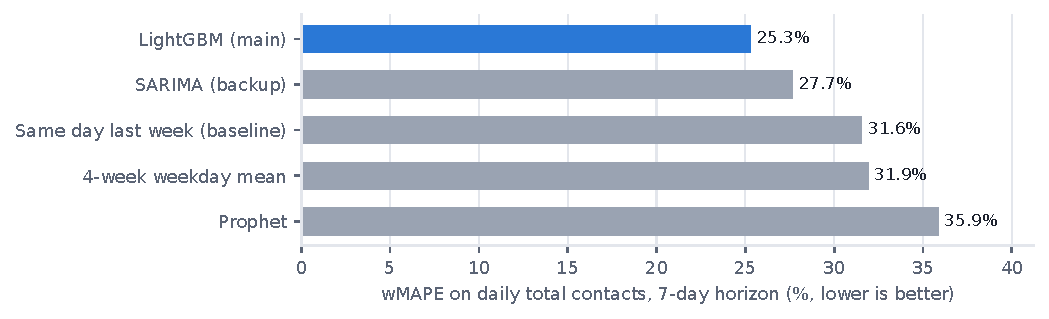
\includegraphics[width=0.86\textwidth]{figures/forecast_wmape.pdf}
\caption{Forecast error on the daily total (rolling backtest, 46 origins, 7-day horizon).}
\label{fig:forecast}
\end{figure}

\begin{table}[!htbp]
\centering\small
\caption{wMAPE (\%) per intent family; lower is better, best in bold.}
\label{tab:forecast}
\begin{tabular}{@{}lrrrrr@{}}
\toprule
\textbf{Family} & \textbf{LightGBM} & \textbf{Same day last week} & \textbf{4-week mean} & \textbf{SARIMA} &
\textbf{Prophet} \\
\midrule
Total & \textbf{25.3} & 31.6 & 31.9 & 27.7 & 35.9 \\
Where is my order & \textbf{36.9} & 45.5 & 48.8 & 42.3 & 52.1 \\
After delivery & 38.0 & 45.1 & 41.9 & \textbf{35.2} & 43.7 \\
Order admin & 54.7 & 68.0 & 55.9 & 53.7 & \textbf{52.7} \\
Cancel / refund & 83.8 & 102.9 & 86.1 & \textbf{81.3} & 90.5 \\
\bottomrule
\end{tabular}
\end{table}

\subsection{DSO4: the twin is faithful}
The twin passes all six fidelity checks (Table~\ref{tab:fidelity}). The first three prove that the engine is
correct (it reproduces Erlang C within 3\%); the last three show it is consistent with its inputs: daily volumes,
hourly profile and handle times are statistically indistinguishable from the history. \textbf{Verdict: kept.}

\begin{table}[!htbp]
\centering\small
\caption{Fidelity of the twin.}
\label{tab:fidelity}
\begin{tabular}{@{}llll@{}}
\toprule
\textbf{Check} & \textbf{Twin} & \textbf{Reference} & \textbf{Rule} \\
\midrule
Erlang C: probability of waiting & 0.279 & 0.285 (error 2.2\%) & error $<$ 5\% \\
Erlang C: mean wait & 33.3 s & 34.2 s (error 2.7\%) & error $<$ 5\% \\
Erlang C: answered within 20 s & 76.5\% & 75.9\% (error 0.8\%) & error $<$ 5\% \\
Daily volume vs history (4 weeks) & 491 / day & 488 / day, KS $p$ = 0.998 & $p > 0.05$ \\
Hour-of-day profile & --- & total variation distance 0.015 & $< 0.05$ \\
Handle time vs ticket logs & 273 s & 272 s, KS $p$ = 0.35 & $p > 0.05$ \\
\bottomrule
\end{tabular}
\end{table}

\subsection{BO4: testing a plan before a peak}
For each peak week we compare the plan a manager would build from the normal forecast (\emph{unprepared})
with the plan built after testing the scenario in the twin (\emph{prepared}), on the same customers. Preparing
always protects the service, and every difference is significant (Figure~\ref{fig:bo4}, Table~\ref{tab:bo4}):
understaffed hours fall by 60--84\%, abandonment by 55--78\%, and the mean wait of live customers by 60--82\%.
Preparing costs extra labour, so the money result depends on what a lost customer is worth. With our
assumption of €8, testing first saves \textbf{€6,991 net over the four peak weeks}; it loses €692 in the staff
shortage week, where the break-even value of a lost customer is €12. A repeat contact plus the risk of losing
the customer usually costs more than €6--12, which is why the break-even, not the euro figure, is the robust
result. Running 10 replications of a week takes 4.5--15.6 seconds, so a manager can test many options.

\begin{figure}[!htbp]
\centering
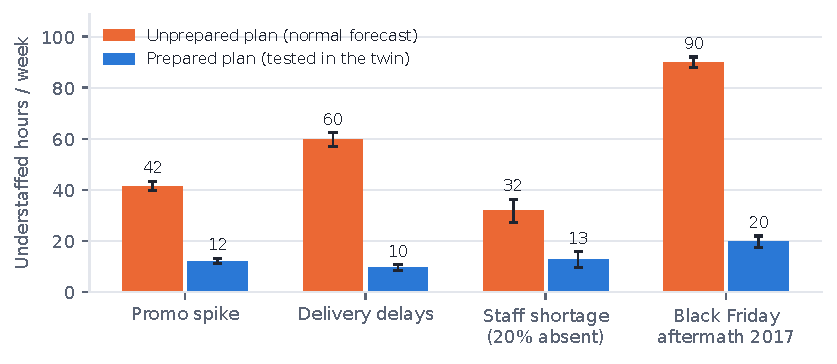
\includegraphics[width=0.86\textwidth]{figures/bo4_understaffed.pdf}
\caption{Understaffed hours per peak week, unprepared vs prepared plan (mean of 10 seeds, 95\% CI).}
\label{fig:bo4}
\end{figure}

\begin{table}[!htbp]
\centering\small
\caption{Testing first, per peak week (unprepared $\rightarrow$ prepared, 10 seeds). Net saving = avoided
lost-customer cost minus extra labour, with its 95\% CI.}
\label{tab:bo4}
\begin{tabularx}{\textwidth}{@{}Yllrr@{}}
\toprule
\textbf{Scenario} & \textbf{Answered $<$ 20 s} & \textbf{Abandonment} & \textbf{Net saving (€)} & \textbf{Break-even} \\
\midrule
Promo spike & 76.1\% $\rightarrow$ 91.9\% & 11.7\% $\rightarrow$ 4.5\% & +226 [129; 323] & €7.4 \\
Delivery delays & 67.8\% $\rightarrow$ 93.7\% & 15.5\% $\rightarrow$ 3.8\% & +1,196 [935; 1,458] & €6.2 \\
Staff shortage (20\% absent) & 81.6\% $\rightarrow$ 92.6\% & 9.8\% $\rightarrow$ 4.4\% & $-$692 [$-$987; $-$397] & €12.1 \\
Black Friday aftermath 2017 & 45.0\% $\rightarrow$ 87.2\% & 29.0\% $\rightarrow$ 6.4\% & +6,261 [5,985; 6,538] & €3.0 \\
\bottomrule
\end{tabularx}
\end{table}

\subsection{DSO3: CP-SAT planning}
In a normal week the CP-SAT plan costs \textbf{€7,050}, against €11,760 for a schedule sized for the busiest
hour (\textbf{$-$40\%}), and still answers 92.4\% of chats within 20 s, above the 80\% target, with every labour
rule respected (Figure~\ref{fig:dso3}). The cost per handled contact falls from €3.20 to €1.95. The rule-based
backup (Erlang C with two shift templates) saves 17\%. In the promotion week, CP-SAT costs €9,762 against
€16,464 (\textbf{$-$41\%}) at 91.9\% service. \textbf{Verdict: main idea kept} ($\geq$5\% cheaper at the target).
A fixed schedule \emph{tuned by hand} to the right level costs about the same in a normal week, because the
Olist hourly profile is flat from 10:00 to 22:00; CP-SAT's value is that it finds this level automatically for
every week and scenario, guarantees the requirement hour by hour and the labour rules, and adapts when demand
has peaks.

\begin{figure}[!htbp]
\centering
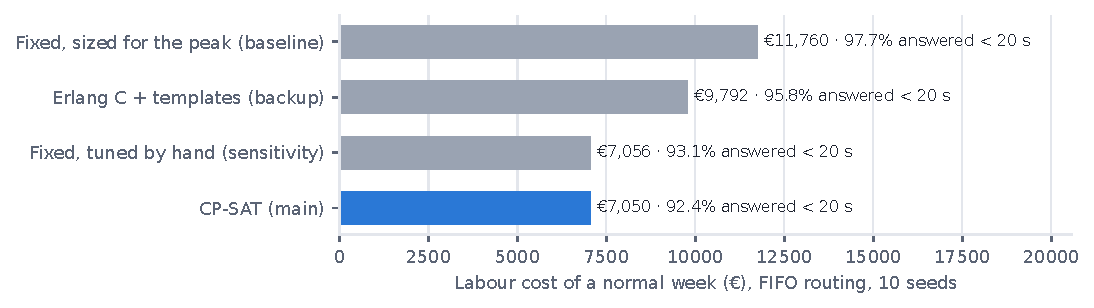
\includegraphics[width=0.86\textwidth]{figures/dso3_planners.pdf}
\caption{Weekly labour cost of the four planners in a normal week, with the service level each one reaches.}
\label{fig:dso3}
\end{figure}

\subsection{DSO1: routing}
On \textbf{unseen stressed days}, both routers beat FIFO significantly (Table~\ref{tab:dso1}): PPO cuts the speed
of answer by \textbf{13.9\%} and raises the service level by 3.4 points; the tuned skill score cuts the mean wait
of live customers by 11.6\% and abandonment by 7.2\%. In the \textbf{full peak weeks} the picture changes
(Figure~\ref{fig:dso1}): neither router changes the mean wait significantly; both reduce abandonment
significantly (skill score $-$6.5\% to $-$9.6\%, PPO $-$3.7\% to $-$4.5\%), and PPO cuts the
90th-percentile wait by 18--25\%. PPO serves customers who have waited long or are about to leave: a fairness
gain that the mean hides. Peak weeks differ from the training days (a backlog that carries over several days,
planned overtime), and PPO was trained on single days.
\textbf{Verdict (switch rule): not met}: the $\geq$10\% gain does not hold in peak weeks. The tuned skill score
is the production candidate (robust, explainable), and PPO stays the research track.

\begin{table}[!htbp]
\centering\small
\caption{Routing on 20 unseen stressed days (40 paired runs). In brackets: change vs FIFO; all significant.}
\label{tab:dso1}
\setlength{\tabcolsep}{4pt}
\begin{tabular}{@{}lllll@{}}
\toprule
\textbf{Router} & \textbf{ASA} & \textbf{Mean wait (all live)} & \textbf{$<$ 20 s} & \textbf{Abandonment} \\
\midrule
FIFO + skill matching (baseline) & 25.2 s & 37.5 s & 59.7\% & 19.7\% \\
Tuned skill score (backup) & 22.6 s ($-$10.3\%) & 33.1 s ($-$11.6\%) & 62.2\% & 18.3\% ($-$7.2\%) \\
MaskablePPO (main) & 21.7 s ($-$13.9\%) & 35.4 s ($-$5.6\%) & 63.0\% & 18.8\% ($-$4.6\%) \\
\bottomrule
\end{tabular}
\end{table}

\begin{figure}[!htbp]
\centering
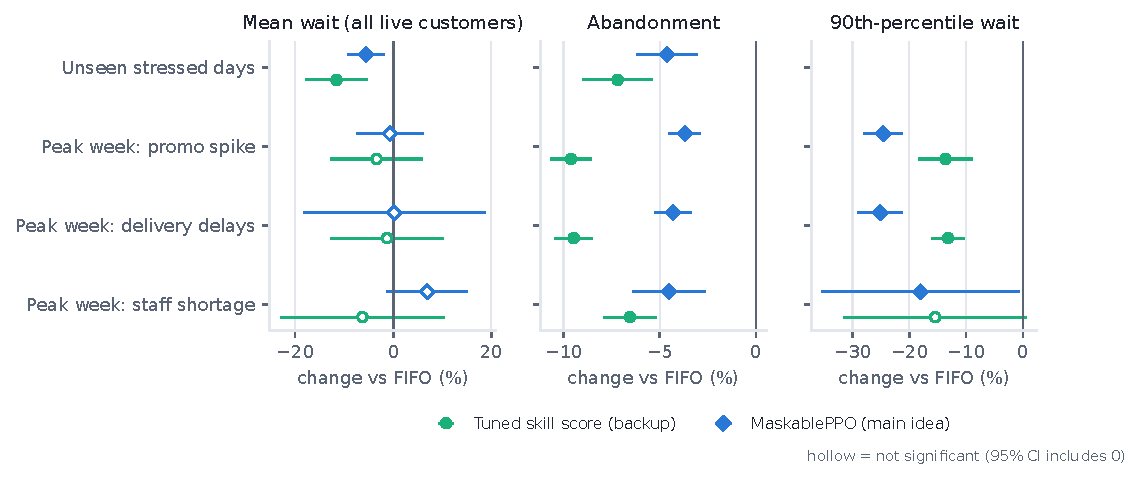
\includegraphics[width=0.98\textwidth]{figures/dso1_routing.pdf}
\caption{Change vs FIFO with 95\% CI. Filled markers are significant; hollow ones are not (the 90th-percentile
wait was not measured in the stressed-day study).}
\label{fig:dso1}
\end{figure}

\subsection{DSO2: retrieval, answers and the judge}
\textbf{Retrieval.} On 255 questions, bge-m3 + FAISS finds the right policy section first 80.0\% of the time and in
the top 4 \textbf{96.9\%} of the time, against 52.9\% and 80.4\% for keyword search (Figure~\ref{fig:retrieval}).
The gap is largest in French (34 questions: 94\% vs 15\% at rank 1), because the embeddings are multilingual.
\textbf{Verdict: retrieval beats the baseline.}

\begin{figure}[!htbp]
\centering
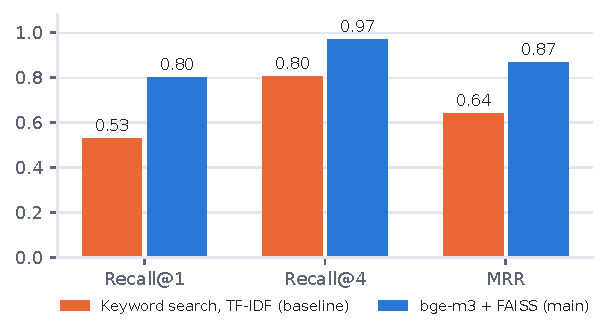
\includegraphics[width=0.62\textwidth]{figures/dso2_retrieval.pdf}
\caption{Retrieval on 255 Bitext questions (17 intents).}
\label{fig:retrieval}
\end{figure}

\textbf{Answers.} Table~\ref{tab:dso2} compares the variants on the same 12 customers. This paired batch was run
on 19--20 October with our first local models (Qwen2.5-3B advisor and client, Llama-3.2-3B judge); the template
variant was later re-run on 40 customers.
The pure RAG advisor writes well-grounded answers (faithfulness 0.99), but nothing in them can be
\emph{verified} as the policy action, and the judge accepted none of them. The hybrid, where the rules engine
decides and the LLM writes, gives a checkable action that is right in \textbf{12/12} chats and the best customer
satisfaction (\textbf{4.33/5}); in 4 of the 12 chats a safety net replaced an LLM draft by the approved text.
Tool calls worked 100\% of the time once tool gating was in place (48\% before).

\begin{table}[!htbp]
\centering\small
\caption{Advisor variants (BO2 KPIs). ``Verified'' compares the advisor's action with the rules' action; the
template variant is judged by the checklist, the LLM variants by the LLM judge.}
\label{tab:dso2}
\setlength{\tabcolsep}{4pt}
\begin{tabular}{@{}lrrrrrr@{}}
\toprule
\textbf{Variant} & \textbf{Chats} & \textbf{Verified} & \textbf{Judge: correct} & \textbf{CSAT} &
\textbf{Faithful.} & \textbf{Similarity} \\
\midrule
Template (backup) & 40 & 100\% & 100\% & 3.83 & 0.65 & 1.00 \\
Pure RAG (idea A) & 12 & not verifiable & 0\% & 3.58 & 0.99 & 0.74 \\
RAG + rules engine (hybrid) & 12 & \textbf{100\%} & 17\% & \textbf{4.33} & 0.70 & 0.79 \\
\bottomrule
\end{tabular}
\end{table}

\textbf{The judge.} Against labels on 60 historical chats, neither judge reaches the 0.4 kappa needed to be
trusted (Table~\ref{tab:judge}). The 3B LLM judge is close to chance; the checklist is better on resolution
(kappa 0.39, Spearman 0.50). Two reasons: a 3B judge is too weak (it called policy-correct answers ``invented
promises''), and the labels are proxies (a generator's answer key), so the satisfaction labels are partly
random. \textbf{Verdict: the AI reviewer is not trusted yet}; the deterministic action check is the
production quality signal, and the judge is advisory.

\begin{table}[!htbp]
\centering\small
\caption{Judge calibration: quadratic weighted kappa on 60 chats (trusted from 0.4).}
\label{tab:judge}
\begin{tabular}{@{}lrrr@{}}
\toprule
\textbf{Judge} & \textbf{Satisfaction} & \textbf{Resolution} & \textbf{Within $\pm$1 point} \\
\midrule
LLM judge (Llama-3.2-3B) & 0.06 & 0.06 & 58--65\% \\
Checklist reviewer (backup) & 0.07 & \textbf{0.39} & 63--65\% \\
\bottomrule
\end{tabular}
\end{table}

\textbf{Tool calling.} Making the LLM choose tools taught us more than any score. SmolLM3-3B never emitted a real
tool call on its own (0 of 186 traced advisor calls); it even \emph{narrated} fake calls (``I've called
lookup\_order...'') with invented facts. Forcing a tool call at the investigation step (the reply is pre-started
with the tool-call marker) gave 6 of 6 real calls with the right order id. The hosted Nemotron models call tools
correctly in about 1.5 s. On the client side, the customer's \code{view\_my\_order\_page} tool caught a wrong
``delivered'' claim by the advisor in a trial.

\subsection{Monitoring the AI components}
\label{sec:monitoring}
Over the 1,339 traced LLM calls and 219 saved chats (live and evaluation, all periods), the monitoring page
(Figure~\ref{fig:monitoringpage}) gives a sober picture (Figures~\ref{fig:latency} and~\ref{fig:confidence}):

\begin{figure}[!htbp]
\centering
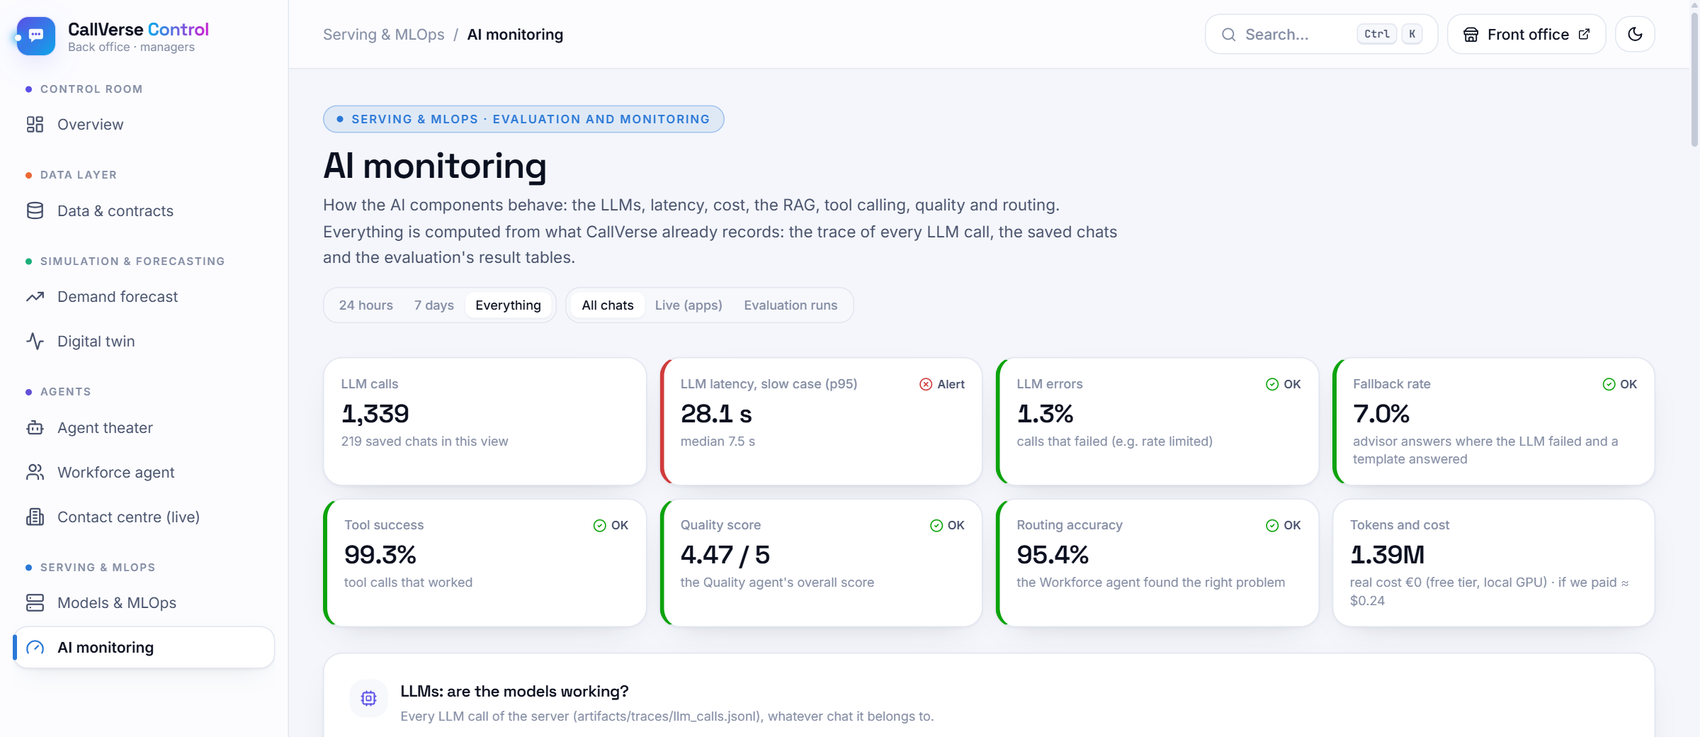
\includegraphics[width=\textwidth]{figures/screen_monitoring.png}
\caption{The AI monitoring page of the back office (all periods, all chats). Each headline indicator turns
amber or red past its threshold, always with an icon and a word (OK, Watch, Alert) as well as a colour.}
\label{fig:monitoringpage}
\end{figure}

\begin{itemize}
  \item \textbf{Latency.} The p95 latency is 28 s (red), but it comes from the local-GPU period: the local
        SmolLM3 advisor answers in 16.2 s at the median (p95 43.1 s), the hosted Nemotron 3.5 Super advisor in
        2.0 s (p95 8.0 s). This measurement drove the switch to OpenRouter.
  \item \textbf{Fallbacks and tools.} 7.0\% of the advisor's LLM answers fell back to a template (amber threshold:
        20\%), and 99.3\% of the tool calls succeeded. Of the tool calls whose caller is recorded, 132 were made by
        fixed pipeline steps and only 13 were chosen by the LLM: the system is honest ``workflow plus agent'', not
        a fully autonomous agent.
  \item \textbf{Routing.} The Workforce agent found the right problem in 95.4\% of the chats; its confidence can
        be trusted: 99.5\% right when it is above 0.9 (186 chats), 78\% between 0.5 and 0.7. The main confusion is
        \code{track\_order} vs \code{track\_delivery} (6 chats), two close intents of the same family (where is my order).
  \item \textbf{Judge vs customer.} The judge's score and the customer's CSAT correlate only weakly (Pearson 0.21),
        another sign that the judge is not yet a reliable proxy.
  \item \textbf{Cost.} The real cost is €0 (free tier and local GPU). At the reference price, the 1.39 million
        tokens would cost \$0.24, about \$0.0002 per resolved chat; 90.9\% of the chats were resolved.
\end{itemize}

\begin{figure}[!htbp]
\centering
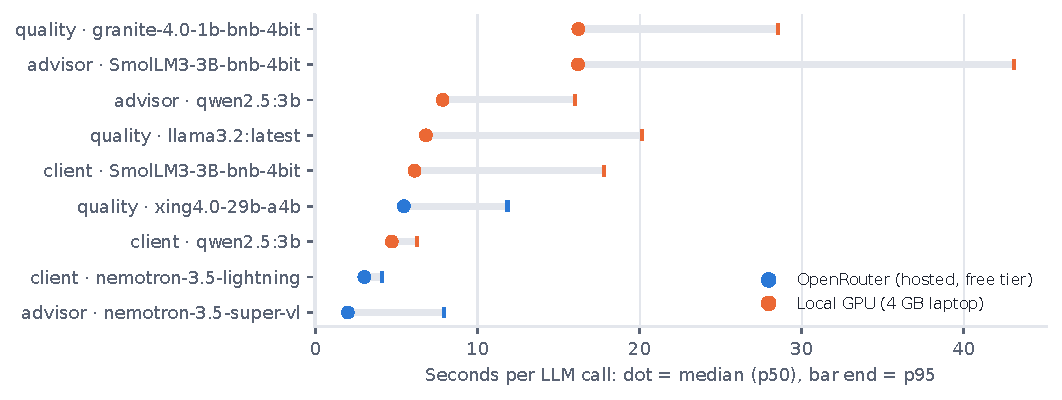
\includegraphics[width=0.86\textwidth]{figures/llm_latency.pdf}
\caption{Latency per LLM call by agent and model (models with at least 10 calls).}
\label{fig:latency}
\end{figure}

\begin{figure}[!htbp]
\centering
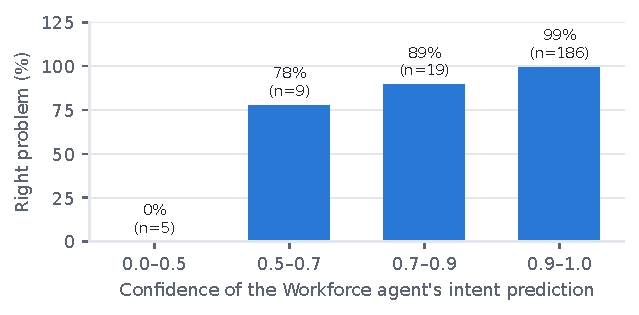
\includegraphics[width=0.6\textwidth]{figures/routing_confidence.pdf}
\caption{Routing accuracy by confidence of the intent prediction (219 chats).}
\label{fig:confidence}
\end{figure}

\subsection{Scorecard}
Table~\ref{tab:scorecard} applies the switch rules. The foundation (DSO4) and the planning objective (DSO3) pass
clearly. DSO1 and DSO2 bring measurable gains, but our own rules put the backup or a hybrid in production.

\begin{table}[!htbp]
\centering\small
\caption{BO/DSO scorecard (\code{artifacts/evaluations/scorecard.json}).}
\label{tab:scorecard}
\begin{tabularx}{\textwidth}{@{}lYcY@{}}
\toprule
\textbf{DSO} & \textbf{Result} & \textbf{Rule met} & \textbf{In production} \\
\midrule
DSO1 routing & PPO: ASA $-$13.9\% on stressed days; in peak weeks mean wait not significant, abandonment
  $-$4\% & no & Tuned skill score \\
DSO2 advisor + judge & Recall@4 96.9\%; hybrid 12/12 verified actions, CSAT 4.33; judge kappa $<$ 0.4 & no &
  Hybrid advisor; template backup; checklist reviewer \\
DSO3 planning & Labour cost $-$40\% at 92.4\% service; labour rules respected & yes & CP-SAT \\
DSO4 forecast + twin & wMAPE 25.3\% vs 31.6\%; all fidelity checks pass; €6,991 net saved over 4 peak weeks &
  yes & LightGBM + twin \\
\bottomrule
\end{tabularx}
\end{table}

\section{Critical analysis and limitations}
\label{sec:analysis}

\paragraph{What the evidence supports.} The strongest results are the ones with the most data and the simplest
claims: the forecast beats its baseline over 46 origins, the engine reproduces queueing theory, and planning
and testing first show large, significant effects over 10 seeds. Where the AI ideas did not meet their own
rule (routing in peak weeks, the judge), the project shipped the backup or a hybrid instead of hiding the
result. We see this discipline (a baseline, a confidence interval and a fallback for every claim) as the main
methodological result.

\paragraph{1. Synthetic contacts.} Contacts, tickets and chats are generated from real orders with assumed
rates, handle times and patience. The twin's agreement with the ``history'' is therefore partly circular: it
shows consistency with its inputs, not with a real centre. The euro amounts depend on our cost assumptions
(€12 per hour, €8 per lost customer); this is why we report break-even values. The pipeline accepts a client's
real logs unchanged, and the fidelity checks would then become a real calibration.

\paragraph{2. Reinforcement learning does not transfer.} PPO was trained on single busy days, but peak weeks
carry a backlog over several days and use planned overtime. It wins on the conditions it was trained for and
loses its mean-wait advantage elsewhere. Its policy is also hard to explain to a planner, while the skill score
has four readable weights. Training on multi-day episodes that match the scenarios is the obvious next step.

\paragraph{3. Small language models invent facts.} The 3B models invented order ids, narrated tool calls they
never made, and the simulated customer sometimes swapped roles with the advisor. Our answer was architectural: \emph{the rules engine
decides, the LLM writes}, tool gating, and safety nets. This works (12/12 verified actions), but it also means
that the system is mostly a workflow: only 13 of the 145 tool calls with a recorded caller were chosen by the
LLM. Larger hosted models call tools correctly, so autonomy can grow as models improve, but every new
autonomous step needs its own measurement.

\paragraph{4. The automatic judge is not trusted.} Kappa stays below 0.4 for both judges, and the judge's score
correlates only weakly with the customer's (0.21). Part of the problem is the judge (a 3B model), part is the
labels (proxies from the generator). The calibration code switches to real human grades as soon as 20 exist
(target 60); collecting them is the main open item, and until then the deterministic action check is the
quality signal.

\paragraph{5. The DSO2 sample is small and dated.} The paired conversation batch covers 12 customers, too few
for tight intervals, and it was run with our first local models (Qwen2.5-3B, Llama-3.2-3B), which the project
no longer uses. Re-running it on the hosted models is limited by the free tier (50 requests per day, while one
conversation takes a few dozen calls). The monitoring numbers cover the current models, but not as a paired
experiment.

\paragraph{6. Dependence on a free hosted service.} OpenRouter's free models are fast and cost nothing, but they
are rate-limited, their availability varies, and, unlike local models, the conversation text leaves the
machine. Our three-tier design (hosted, local, templates) keeps the twin working when the quota runs out, at
the price of simpler answers.

\paragraph{7. Scope of the twin.} One channel (chat), one queue per family, four problem families and Brazilian
e-commerce only. Real centres mix voice, e-mail and chat and route by language and seniority. The phone page
of the application is a live demonstration, not a channel modelled in the simulation.

\paragraph{8. Metrics have limits too.} Our faithfulness measure is an embedding similarity, a cheap local
stand-in for an LLM-graded RAGAS; it scores templates low only because formatted dates do not match raw JSON
fields. In a normal week, a hand-tuned fixed schedule costs as little as CP-SAT, because the Olist hourly
profile is flat: CP-SAT's advantage is automation and guarantees, not a lower cost in every week.

\paragraph{What we would do differently.} Collect a small set of real, human-labelled chats early, to calibrate
the judge before building on it; decide the LLM provider earlier, since the move from local to hosted models
came late and left the DSO2 batch on old models; and train the RL router on the same multi-day episodes that
the evaluation uses.

\section{Deployment and reproducibility}
\label{sec:deployment}

\subsection{The application}
One FastAPI~\cite{fastapi} backend serves two React applications (Figure~\ref{fig:screens}):
\begin{itemize}
  \item the \textbf{front office}, for customers and advisors: a help centre with semantic search, demo
        customers on real Olist orders, a live chat with the AI advisor (streamed word by word, with a
        ``behind the scenes'' trace of every agent, tool and policy section, then a satisfaction survey and the
        quality review), an advisor desk (queue, copilot drafts, autopilot), voice input through the browser's
        speech recognition, and a phone page;
  \item the \textbf{back office}, for managers: data and contracts, the forecast, the digital twin (a live floor
        that replays a simulated day contact by contact, and a scenario lab), the agent theatre, workforce
        planning, models and MLOps, the \textbf{AI monitoring} page (Section~\ref{sec:monitoring}), and a
        full-screen \textbf{live contact centre} (Figure~\ref{fig:centre}) where every move of the animated
        staff is a real event: a customer walks in (an AI customer, an existing customer or a new one with a
        new problem), the receptionist (Workforce agent) routes the chat, the advisor answers with tool badges
        in its speech bubbles, and the quality lead posts the score. Real chats from the portal or the phone
        appear there too, and each person can speak their lines aloud.
\end{itemize}

\begin{figure}[!htbp]
\centering
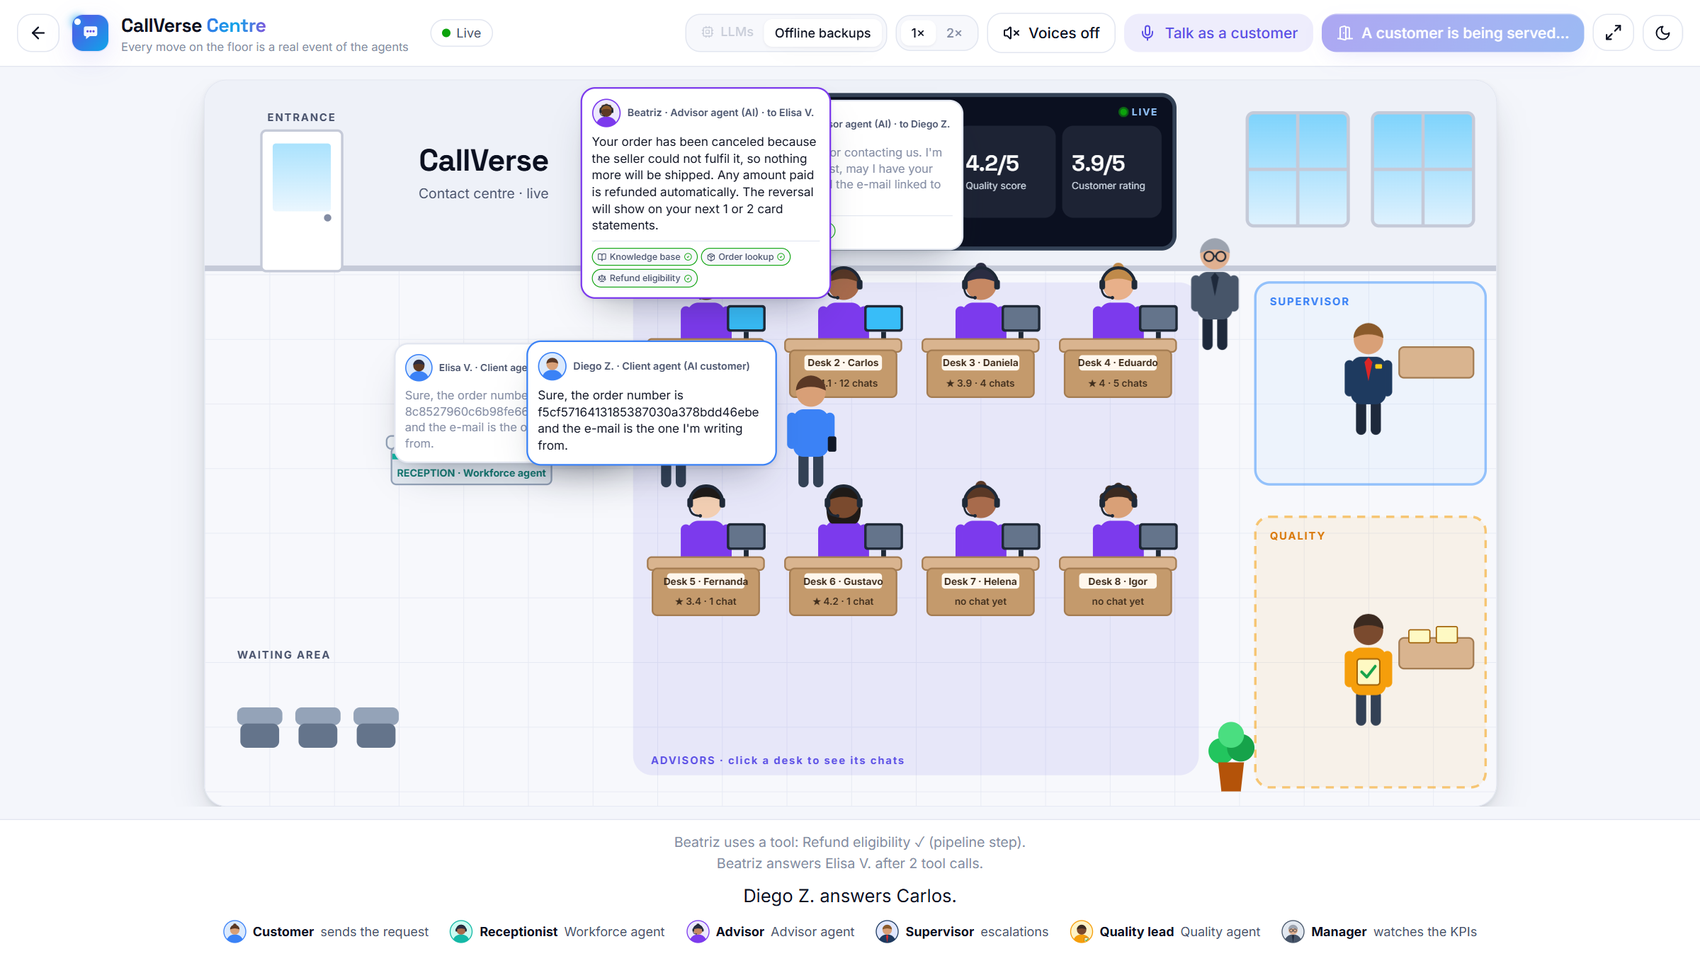
\includegraphics[width=\textwidth]{figures/screen_centre.png}
\caption{The live contact centre (back office, full screen), here with the offline templates. Two AI customers
were routed by the Workforce agent to desks 1 and 2. Beatriz's answer carries the badges of the tools behind it
(knowledge base, order lookup, refund eligibility); the footer narrates each real event, such as ``Beatriz uses
a tool: Refund eligibility (pipeline step)''.}
\label{fig:centre}
\end{figure}
The live chat and the contact centre use WebSockets. The API is documented with OpenAPI at \code{/docs}, and an
MCP server exposes the business tools to outside AI applications (stdio or \code{/mcp} over HTTP).

\begin{figure}[!htbp]
\centering
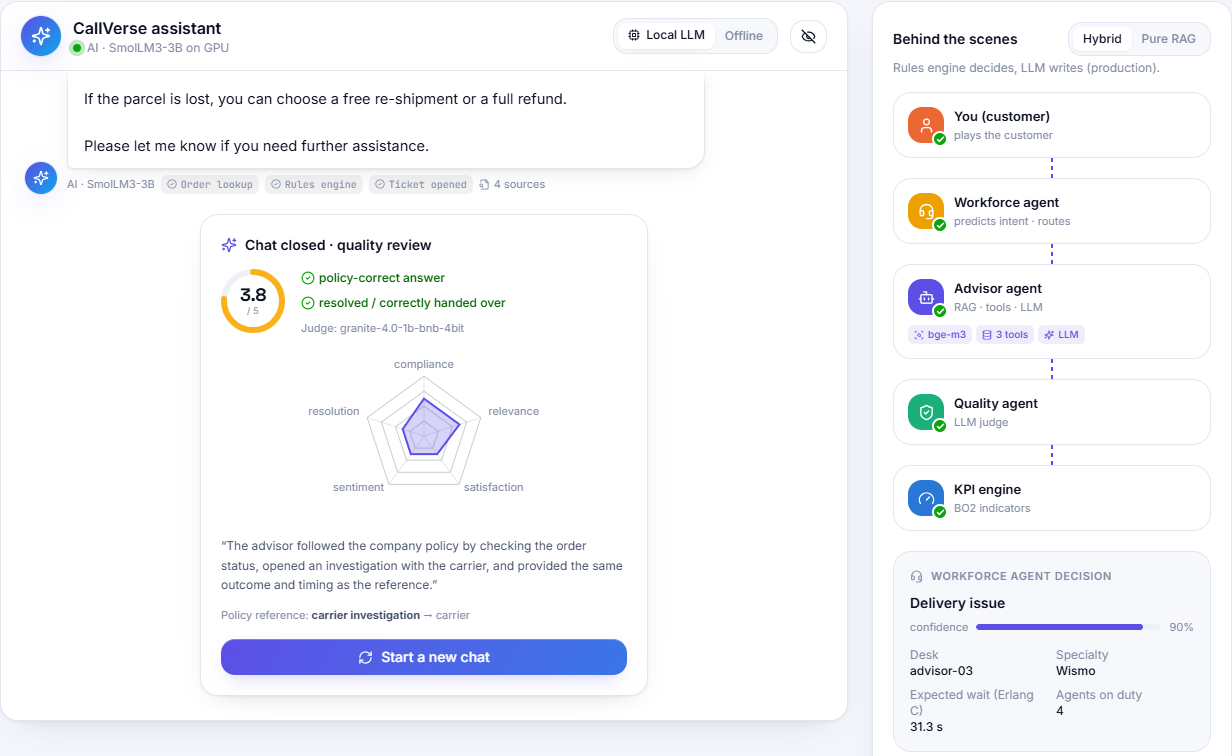
\includegraphics[width=0.53\textwidth]{figures/screen_chat_review.png}\hfill
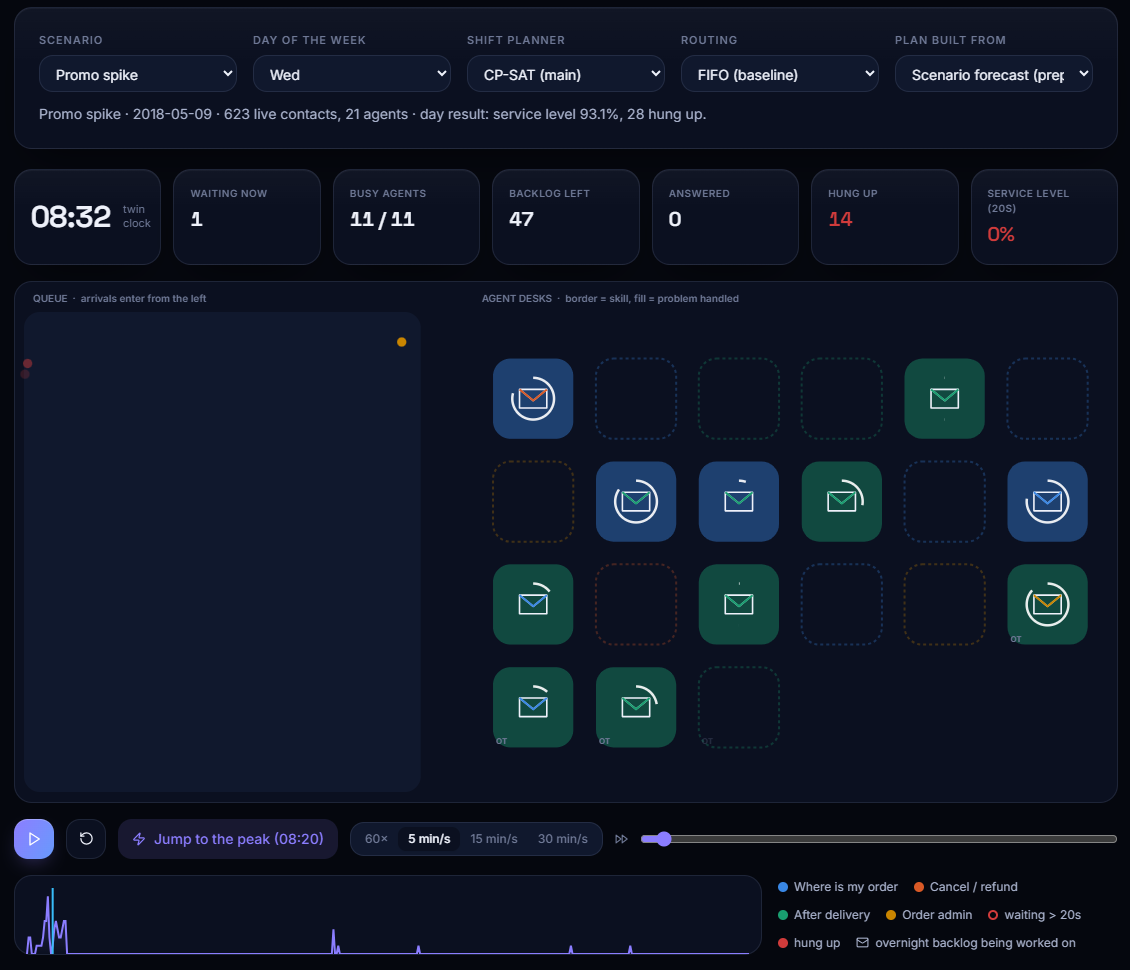
\includegraphics[width=0.44\textwidth]{figures/screen_twin_floor.png}
\caption{Left: the front office after a chat, with the quality review and the ``behind the scenes'' trace
(captured on 1 November 2026, in the local-model period). Right: the twin's live floor replaying a promotion
day with a CP-SAT plan.}
\label{fig:screens}
\end{figure}

\subsection{One container}
The whole application ships as \textbf{one Docker image}. A first stage builds the two React apps with Node; a
second stage installs the Python package on Python 3.12 and serves both apps from the API: the front office at
\code{/}, the back office at \code{/back-office/}, the API at \code{/api}, \code{/ws}, \code{/docs} and
\code{/mcp}. Three details make the image reproducible: the library versions are pinned to those of the
environment that trained the saved models (\code{space/constraints.txt}, 31 libraries, so the scikit-learn
classifier, the PPO policy and the MLflow database load unchanged); the bge-m3 model is downloaded at build time
and the build fails if it cannot load \emph{offline}; and the Linux builds of the JavaScript build tools are
added, because the lock file was produced on Windows. For local use, Docker Compose also runs MLflow with
PostgreSQL and an nginx front.

\subsection{Online deployment}
Our first target was Hugging Face Spaces, which used to host Docker apps for free. On 11 November 2026 the
platform answered that Docker Spaces now require a paid subscription (HTTP 402), so we deploy on
\textbf{Azure for Students}. Its credit-only subscriptions cannot run cloud image builds (ACR Tasks), and
pushing a 6 GB image over our connection would take hours. We therefore use a small Linux virtual machine
(Ubuntu 24.04, 2 vCPUs, 8 GB): \code{scripts/deploy\_azure.py} sends only a cleaned build folder (about 120 MB
compressed), the VM downloads the heavy parts and builds the image itself, and a Caddy container in front
obtains a free Let's Encrypt certificate. HTTPS is required for the microphone and for secure WebSockets.
The demo runs at \demourl.

Before anything leaves the laptop, the deployment script copies an \emph{allowlist} of files (never \code{.env},
keys or caches), deletes the customers we created while testing (our own names) from the copied database and
compacts it, so the deleted rows cannot be recovered, leaves out our live chat transcripts, keeps only the
numbers of the LLM trace, and stops if it finds a secret or one of the removed names. The OpenRouter key goes to
the VM through SSH input into a file only the service user can read. The public demo has no login, and visitor
data is reset at each deployment: it is a demonstration, not a production service.

\subsection{Reproducibility and code quality}
\begin{itemize}
  \item \textbf{One command per stage}: \code{callverse all} runs the whole pipeline (data, contracts,
        forecast, RL training, experiments, scorecard); \code{callverse evaluate} re-runs every experiment of
        Section~\ref{sec:experiments}. Notebooks are executed headless and their outputs archived.
  \item \textbf{Fixed randomness}: seeds live in \code{configs/}; experiments use common random numbers; CP-SAT runs
        on one thread so that the roster does not change between runs.
  \item \textbf{Pinned models and versions}: Hugging Face commits are recorded (\code{llm\_models.lock.json}),
        LLM answers are cached, and library versions are pinned for deployment.
  \item \textbf{Tracking}: MLflow records the parameters, metrics and artefacts of the forecast, RL and
        evaluation runs; every LLM call is traced.
  \item \textbf{Tests and checks}: 200 automated tests (unit, smoke and integration; they cover every layer,
        including live WebSocket sessions, the contact-centre hub and the serving of the built apps), the
        \code{ruff} linter,
        six import contracts for the layered architecture, and a GitHub Actions workflow that runs them and
        type-checks and builds both web apps.
  \item \textbf{Documentation}: the README (installation, execution, structure), a step-by-step run guide, the
        data reports of every phase, and the experiment protocol.
\end{itemize}

\section{Conclusion and future work}
\label{sec:conclusion}

CallVerse shows that forecasting, discrete-event simulation, optimisation, reinforcement learning and
language-model agents can work together on one business problem: running a customer service centre well.
The foundation clearly beats its baselines: the forecast lowers the error from 31.6\% to 25.3\%, and the twin
reproduces queueing theory and the history. On top of it, CP-SAT planning cuts labour cost by 40\% at the
service target, and testing a plan before a peak cuts understaffed hours by 60--84\%. Routing and AI answering
bring measurable gains, but our own switch rules sent a tuned rule and a hybrid advisor (the rules engine
decides, the LLM writes) to production, while the pure-AI versions remain research tracks. The automatic judge
is not yet trusted, and we say so. The application, from the customer portal to the live contact-centre view
and the monitoring of every AI component, is tested, documented and packaged as one container, ready for online deployment.

\paragraph{Future work.}
\begin{itemize}
  \item \textbf{Real data}: calibrate contact rates, handle times and patience on a partner's logs, and turn the
        fidelity checks into a real calibration.
  \item \textbf{Human labels}: grade 60 real conversations to calibrate the judge, then try a stronger hosted
        judge from another model family.
  \item \textbf{Routing}: train PPO on multi-day episodes matching the peak scenarios, and compare it with the
        skill score behind an A/B test.
  \item \textbf{Agents}: re-run the paired DSO2 batch on the hosted models with a larger sample, and widen the
        LLM's own tool choices step by step, each with its measurement.
  \item \textbf{Monitoring}: add a chat inspector timeline, drift detection on the incoming intents, a safety
        test set, and a one-click regression run before each deployment.
  \item \textbf{Product}: more channels in the twin (voice, e-mail), connectors to help-desk tools, and
        authentication for the online application.
\end{itemize}

\section{Declaration of the use of generative AI tools}
\label{sec:aiuse}

As required by the assessment rules, we declare the generative AI tools used in this project.

\begin{itemize}
  \item \textbf{Claude (Anthropic), through Claude Code}, was used as a programming and writing assistant
        throughout the project: to write and refactor code and tests, to build the web interfaces, to write the
        documentation and the deployment scripts, and to draft this report from our documentation and result
        files. The figures of this report are drawn by a script (\code{report/make\_figures.py}) directly from
        the result tables, and every number comes from those tables or from the project's reports.
  \item \textbf{Our own responsibility.} We chose the problem, the objectives and the switch rules, made the
        design decisions, ran the experiments, checked the results and reviewed every section. Every result can
        be reproduced with the commands of Section~\ref{sec:deployment}.
  \item \textbf{Language models inside the product} are part of the system studied, not tools used to write it:
        NVIDIA Nemotron 3.5 and Xing 4.0 (through OpenRouter), SmolLM3-3B and IBM Granite-4.0-1B (local), and,
        in the first experiments, Qwen2.5 and Llama 3.2. They are described in Section~\ref{sec:llmsetup}.
\end{itemize}


{\small
\bibliographystyle{plain}
\bibliography{references}
}

\end{document}
